\begin{frame}
    \frametitle{Entities}
    
    A manuscript or a print (\textbf{Historical Document}) contains a version (\textbf{Witness}) of a story (\textbf{Text}).
    For example, folios in the Venetian manuscript Fr.Z.13 contain parts of the story \textit{Orlandino}.
    
    \tiny
    
    \tikzstyle{arrow} = [thick,->,>=stealth]
    \tikzstyle{block} = [
        rectangle,
        minimum width=2cm,
        minimum height=0.5cm,
        text centered,
        draw=black,
        fill=cyan!30
    ]
    
    \begin{center}
    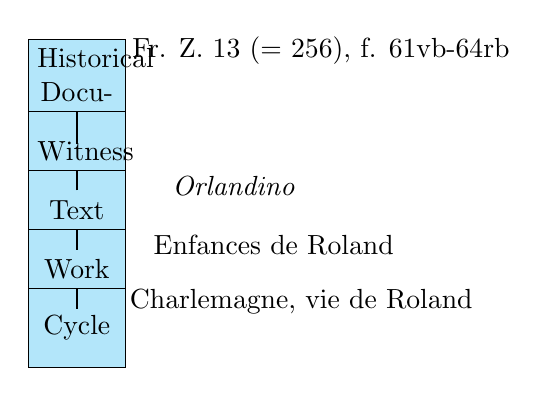
\begin{tikzpicture}[node distance=0.75cm]
        \node (historical) [%
            block,%
            label={
                [xshift=3.1cm, yshift=-0.45cm]
                {Fr. Z. 13 (= 256), f. 61vb‑64rb}
            }%
            ] {Historical Document};
        
        \node (witness) [%
            block,%
            below of=historical
            ] {Witness};
    
        \node (text) [%
            block, %
            below of=witness, %
            label={%
            [xshift=2cm, yshift=-0.45cm]
            {\textit{Orlandino}}%
            }%
            ] {Text};
        
        \node (work) [%
            block,%
            below of=text, %
            label={%
            [xshift=2.5cm, yshift=-0.45cm]
            {Enfances de Roland}%
            }%
            ] {Work};
    
        \node (cycle) [%
            block,%
            below of=work,
            label={%
            [xshift=2.85cm, yshift=-0.45cm]
            Charlemagne, vie de Roland%
            }%
            ] {Cycle};
    
        \draw [arrow] (witness) -- (text);
        \draw [arrow] (text) -- (work);
        \draw [arrow] (work) -- (cycle);
        \draw [arrow] (historical) -- (witness);
    
    \end{tikzpicture}
    \end{center}
    
    \normalsize
    
    The story or \textit{chanson} (\textbf{Text}) fits into a larger tale or \textit{geste} (\textbf{Work}).
    Finally, the larger tale (\textbf{Work}) relates to one or more overarching \textbf{Cycles} of tales.
    For example, the tale about Roland's childhood relates to the \textbf{Cycles} about Roland's life
    and Charlemagne's life.
        
    \end{frame}
    
    \begin{frame}
    \frametitle{Within a Cycle, Works and their Texts}
    
    Within the \textbf{Cycle} \textit{Charlemagne, vie de Charlemagne}, there are 3 known \textbf{Works}:
    the story of Mainet, of Roland's childhood, and of Morant and Galienne.
    Each \textbf{Work} was articulated (has a \textbf{Text}) in at least one language.
    When no surviving \textbf{Witness} exists, the language of the \textbf{Text} might be unknown.
    
    \tiny
    
    \tikzstyle{arrow} = [thick,-,>=stealth]
    \tikzstyle{block} = [
        rectangle,
        minimum width=1cm,
        minimum height=1cm,
        text width=1cm,
        text centered,
        draw=black,
        fill=cyan!30
    ]
    \tikzstyle{bigblock} = [
        rectangle,
        minimum width=2cm,
        minimum height=1cm,
        text width=2cm,
        text centered,
        draw=black,
        fill=cyan!30
    ]
    
        \begin{center}
        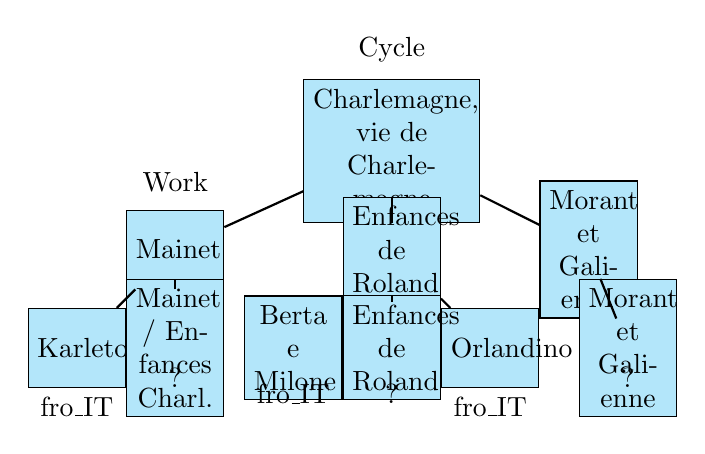
\begin{tikzpicture}[node distance=1.25cm]
            \node (cycle) [%
                bigblock,
                label={
                [yshift=0.1cm]
                {Cycle}
                }
                ] {Charlemagne, vie de Charlemagne};
            \node (enfances) [
                block,
                below of=cycle
            ] {Enfances de Roland};
    
            \node (mainet) [
                block,
                left of=enfances,
                xshift=-1.5cm,
                label={
                [yshift=0.1cm]
                {Work}
                }
            ] {Mainet};
            \node (morant) [
                block,
                right of=enfances,
                xshift=1.25cm
            ] {Morant et Galienne};
    
            \draw [arrow] (mainet) -- (cycle);
            \draw [arrow] (enfances) -- (cycle);
            \draw [arrow] (morant) -- (cycle);
    
            \node (morant_text) [
                block,
                below of=morant,
                xshift=0.5cm,
                label={
                    [yshift=-1.5cm]
                    {?}
                }
            ] {Morant et Galienne};
    
            \draw [arrow] (morant) -- (morant_text);
    
            \node (karleto) [
                block,
                below of=mainet,
                xshift=-1.25cm,
                label={
                    [yshift=-1.5cm]
                    {fro\_IT}
                }
            ] {Karleto};
    
            \node (mainet_text) [
                block,
                below of=mainet,
                label={
                    [yshift=-1.5cm]
                    {?}
                }
            ] {Mainet / Enfances Charl.};
    
            \draw [arrow] (mainet) -- (karleto);
            \draw [arrow] (mainet) -- (mainet_text);
    
            \node (berta) [
                block,
                below of=enfances,
                xshift=-1.25cm,
                label={
                    [yshift=-1.5cm]
                    {fro\_IT}
                }
            ] {Berta e Milone};
    
            \node (orlandino) [
                block,
                below of=enfances,
                xshift=1.25cm,
                label={
                    [yshift=-1.5cm]
                    {fro\_IT}
                }
            ] {Orlandino};
    
            \node (enfances_text) [
                block,
                below of=enfances,
                label={
                    [yshift=-1.5cm]
                    {?}
                }
            ] {Enfances de Roland};
    
            \draw [arrow] (enfances) -- (berta);
            \draw [arrow] (enfances) -- (orlandino);
            \draw [arrow] (enfances) -- (enfances_text);
    
        \end{tikzpicture}
    
        \end{center}
        
    \end{frame}

